\subsection{Architecture}

As anticipated at the beginning, a CNN is used. The architecture of the network is showed in figure \ref{fig:BasicArch}.
\begin{figure}[h!]
	\centering
	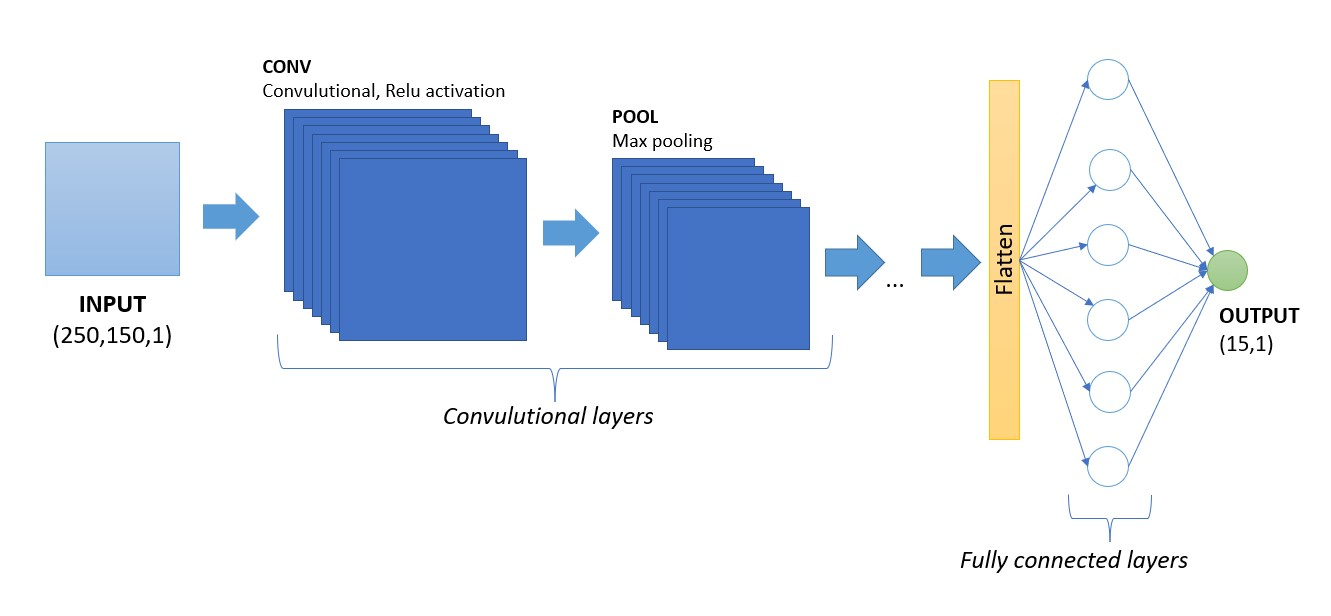
\includegraphics[width=0.7\linewidth]{./ImageFiles/CNN/BasicArch}
	\caption{CNN's basic architecture.}
	\label{fig:BasicArch}
\end{figure}

There is a first convulutional part, formed by three sets of $CON \Rightarrow RELU \Rightarrow MaxPool$. The second part is the classification, given by three fully connected layers activated by RELU.